\documentclass[pdf,11pt]{beamer}

\usepackage[utf8]{inputenc}
\usepackage{graphicx}       % Images
\graphicspath{{Images/}}
\usepackage{xcolor}         % Change Colors
\usepackage{caption}
\captionsetup[figure]{font=small}
\usepackage{multimedia}     % Movies!
\usepackage{tikz}           % Vectored pictures
%\usepackage{media9}
%\hypersetup{pdfpagemode=FullScreen} % Presentation Mode
\usepackage{animate}        % gifs
\usepackage{tikz}
\usepackage{amsmath}
\usepackage{amssymb}
\usepackage{subcaption} % for subfigure
\tikzset{
    ->,
    level distance = 12em,
    minimum size=2em,
    %edge from parent/.style={draw,thick},
    level 1/.style={sibling distance=6em},
    level 2/.style={sibling distance=3em},
    thick/.style = {line width=1.5pt},
    extra thick/.style = {line width=3.5pt},
    red node/.style={shape=circle,draw=red,fill=red!40,thick,inner sep=1.2},
    blue node/.style={shape=circle,draw=blue,fill=blue!40,thick,inner sep=1.2}
}

\tikzstyle{round}=[thick,draw=black,circle]

% Remove navigation symbols
\beamertemplatenavigationsymbolsempty
% Add page number
\addtobeamertemplate{navigation symbols}{}{%
    \usebeamerfont{footline}%
    \usebeamercolor[fg]{footline}%
    \hspace{1em}%
    \insertframenumber/\inserttotalframenumber
}

% Title
\title{UO 631 Parallel Processing:\\Multi-layer Perceptron Classification
}
\author{Luis Guzman \& Steven Walton\\ \small University of Oregon}
\date{3 December 2020}

\usebackgroundtemplate
{
    
\includegraphics[width=\paperwidth,height=\paperheight]{UO_Simple.png}
}
\definecolor{UOYellow}{HTML}{FDCB00}
\definecolor{UOGreen}{HTML}{424443}
%\newcommand{\mytitle}[1]{\setcolor{bg=UOYellow,fg=green}\frametitle{{#1}}}

% Formatting
%\setbeamercolor{title}{fg=white}
%\setbeamercolor{normal text}{fg=white}
%\setbeamercolor{structure}{fg=white}        % Adjusts figures and frame titles
%\setbeamertemplate{frametitle}[default][center]
%\setbeamerfont{frametitle}{size=\Huge}
%%\setbeamerfont{normal text}{size=\LARGE}
%%\setbeamerfont{structure}{size=\LARGE}
%\setbeamercolor{footline}{fg=UOGreen}
%%\setbeamerfont{footline}{series=\bfseries}


\begin{document}
\frame{\titlepage}

%%%%%%%%%%%%%%%%%%%%%%%%%%%%%%
% Use include for new sections
%%%%%%%%%%%%%%%%%%%%%%%%%%%%%%

\begin{frame}
\begin{itemize}
    \item \textbf{\color{red}{What are Multi-Layer Perceptrons}}
    \item Gradient Descent
    \item Code Profiling
    \item CPU Parallelization
    \item GPU Parallelization
    \item Performance Results 
    \item Next Steps
\end{itemize}
\end{frame}



\begin{frame}
\begin{itemize}
    \item What are Multi-Layer Perceptrons
    \item \textbf{\color{red}{Gradient Descent}}
    \item Code Profiling
    \item CPU Parallelization
    \item GPU Parallelization
    \item Performance Results 
    \item Next Steps
\end{itemize}
\end{frame}

\begin{frame}
    \frametitle{Gradient Descent}
    \center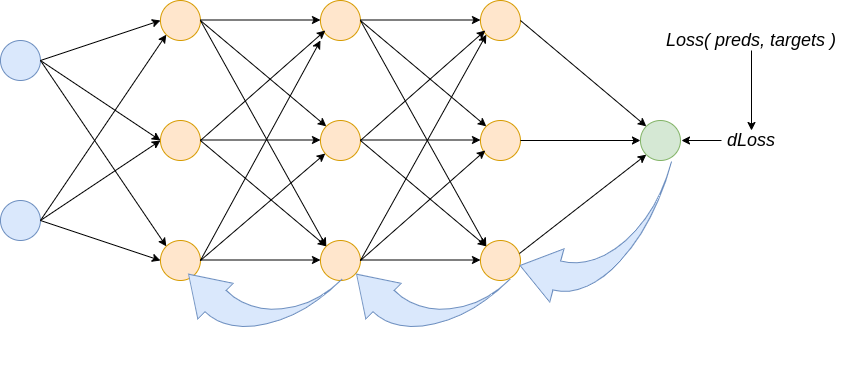
\includegraphics[width=.8\textwidth]{Images/backprop.png}
    \begin{itemize}
        \item $h_{1_{act}} = W_{h_1} * Inputs$
        \item $h_{2_{act}} = W_{h_2} * h_{1_{act}}$
        \item $h_{3_{act}} = W_{h_3} * h_{2_{act}}$
        \item $\hat{y} = W_{O} * h_{3_{act}}$
        \item How do we improve the predictions?
    \end{itemize}
\end{frame}

\begin{frame}
    \frametitle{Back-propagating the error}
    \center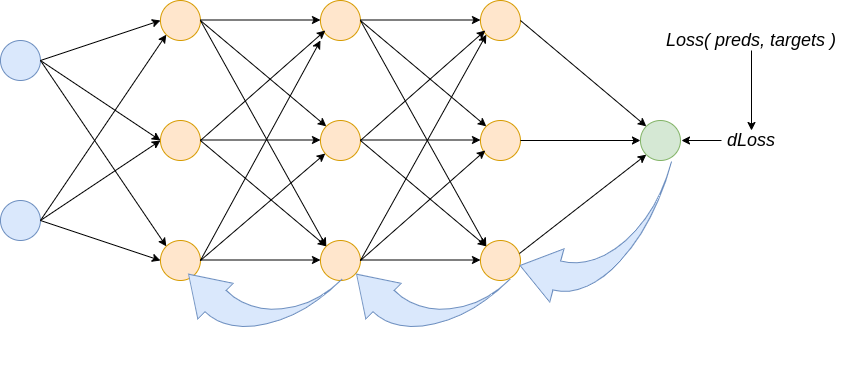
\includegraphics[width=.8\textwidth]{Images/backprop.png}
    \begin{itemize}
        \item $h_{1_{act}} = W_{h_1} * Inputs$
        \item $h_{2_{act}} = W_{h_2} * h_{1_{act}}$
        \item $h_{3_{act}} = W_{h_3} * h_{2_{act}}$
        \item $\hat{y} = W_{O} * h_{3_{act}}$
        \item How do we improve the predictions?
    \end{itemize}
\end{frame}


\begin{frame}
\begin{itemize}
    \item What are Multi-Layer Perceptrons
    \item Gradient Descent
    \item \textbf{\color{red}{Code Profiling}}
    \item CPU Parallelization
    \item GPU Parallelization
    \item Performance Results 
    \item Next Steps
\end{itemize}
\end{frame}



\begin{frame}
\begin{itemize}
    \item What are Multi-Layer Perceptrons
    \item Gradient Descent
    \item Code Profiling
    \item \textbf{\color{red}{CPU Parallelization}}
    \item GPU Parallelization
    \item Performance Results 
    \item Next Steps
\end{itemize}
\end{frame}

\begin{frame}
    \frametitle{CPU Optimization/Parallelization}
    \begin{itemize}
        \item Started with gpof to see what was slowing things down.
        \item Optimized serial version looking to make sure it was memory
            efficient (loops). 
        \item Found the matrix multiplication and transpose were the most heavy
            computation.
    \end{itemize}
\end{frame}

\begin{frame}
    \frametitle{Optimizing Matrix Multiplication}
    \begin{itemize}
        \item Original implementation was not great for parallelization.
        \item Introduced batching.
        \item Found that if the problem was too small parallelization made
            things worse (actually need DNN).
        \item Tried multiple versions of matrix multiply (2 naive and blocking)
    \end{itemize}
\end{frame}

\begin{frame}
    \frametitle{Performance}
    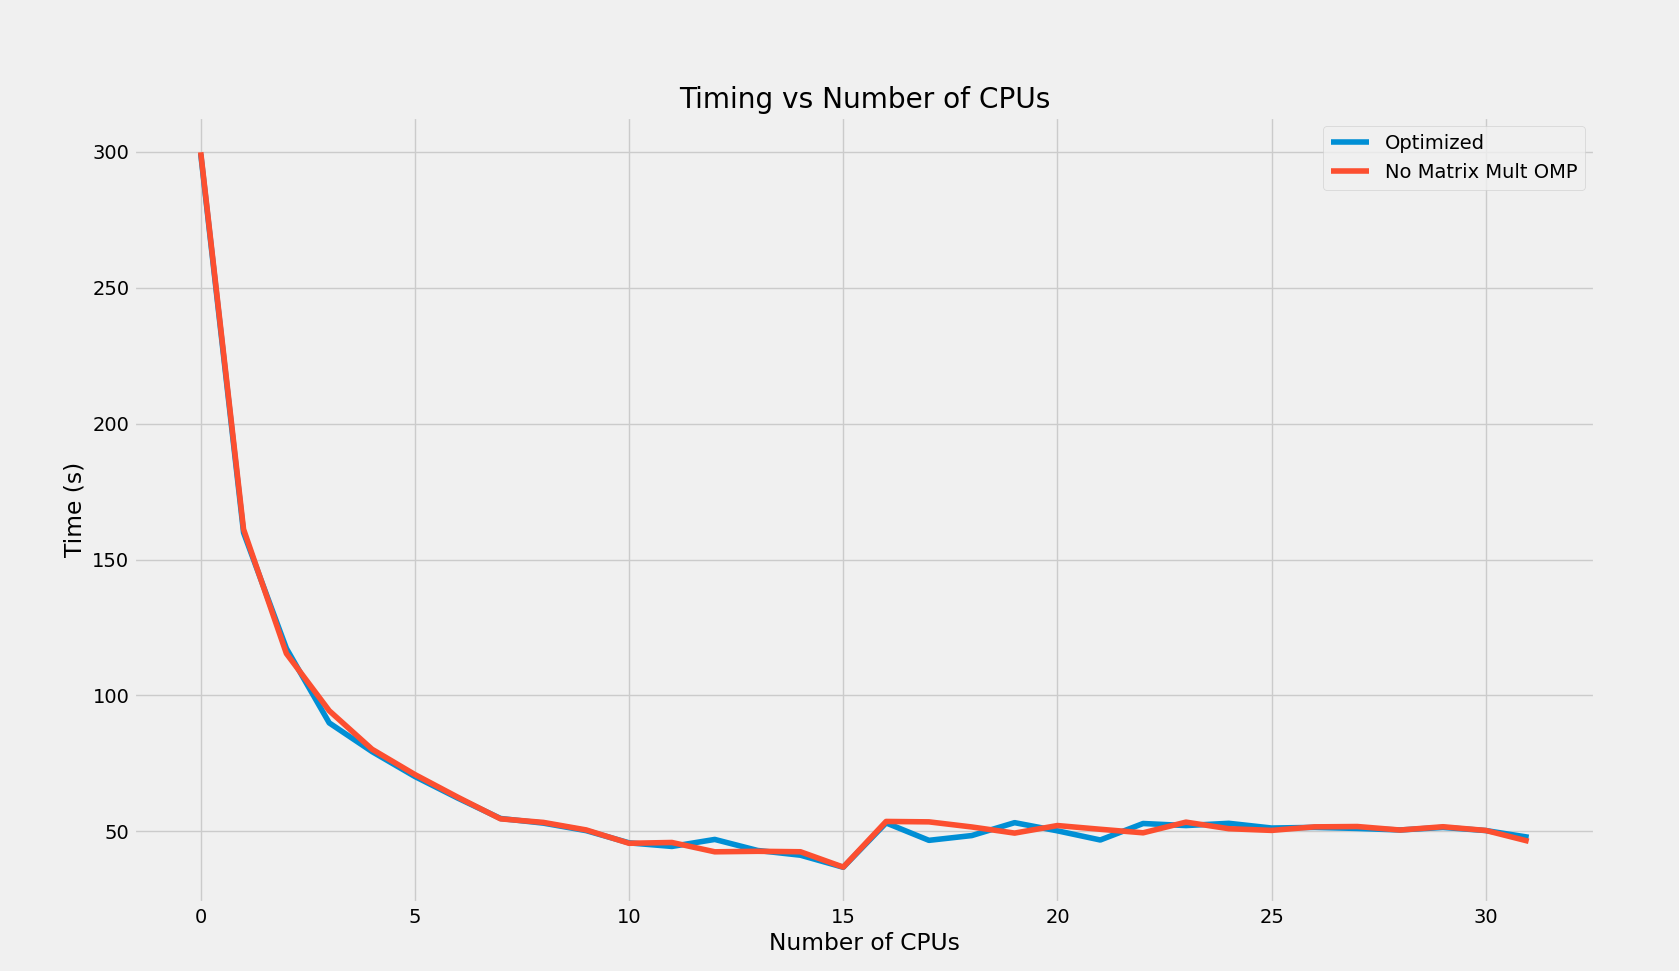
\includegraphics[width=\textwidth]{cpu.png}
\end{frame}





\include{CUDA
\include{NextSteps}

\end{document}
